
\section{Combinatorics on Posets}

Recall $(A, \leq) \subseteq A \times A$.
Instead of $(a,b) \in \, \leq$ we use the notation $a \leq b$. $\leq$ is a partial order if

\begin{tabular}{ll}
  1) $\leq$ reflexive: &
    $\forall x \in A: x \leq x$ \\
  2) $\leq$ transitive:  &
    $\forall x,y,z \in A: x \leq y \land y \leq z \implies x \leq z$ \\
  3) $\leq$ antisymmetric: &
    if $x \leq y \land y \leq x$ then $x = y$ \\
\end{tabular}

$(A,\leq)$ is a poset (partially ordered set).

A poset $(A,\leq)$ is linearly ordered if
\[
  \forall x,y, \in A: x \leq y \lor y \leq x
\]

\textbf{Examples.}\\\\
\begin{tabular}{l l}
  $(\mathbb{N}, \leq), (\mathbb{R}, \leq)$: & Posets, even linearly ordered \\\\

  $(\mathbb{N}^{+}, |)$:
    & $a|a$ \\
    & $ a|b, b|c \implies a|c$\\
    & $ a|b \land b|a \implies a = b$\\
    & Poset, not linearly ordered since $2 \not|~ 3 \land 3 \not|~ 2$\\\\

  $(2^A, \subseteq)$:
    & $ B \subseteq B$\\
    & $ B \subseteq C \subseteq D$\\
    & $ B \subseteq C \land C \subseteq B \implies B = C$ \\
    & Poset, If $|A|\leq 1$ then it is even a linearly ordered poset.
\end{tabular}

\begin{definition}
Given a poset $(A, \leq)$.
An element $x \in A$ is a \dt{minimal element} if $y \leq x \implies x=y$. A linearly ordered set has only one minimal element. Distinct minimal elements of a poset are not comparable:
\begin{align*}
  x,x' \text{ min} &\implies x=x' \text{ or } x,x' \text{ not comparable }\\
  x ≤ x'           &\implies x = x'\\
  x' ≤ x           &\implies x = x'
\end{align*}

Each poset can be visualized by a Hasse diagram.

\begin{center}
    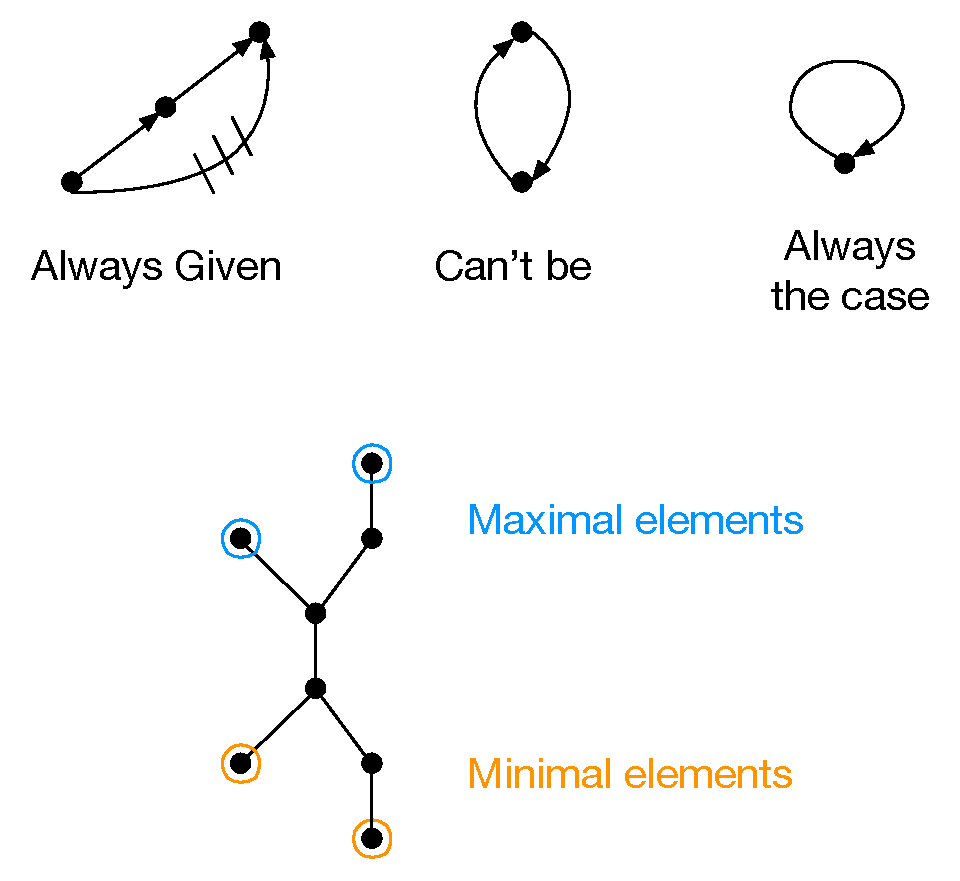
\includegraphics[width=0.6\textwidth]{02_higher_combinatorics/pics/Lattice}
\end{center}

An element $x \in A$ is
\begin{compactitem}
  \item a \dt{maximal element} if $y \geq x \implies x=y$
  \item the \dt{0-element} if $\forall y \in A : x \leq y$ \\
    (every 0-element is minimal)
  \item the \dt{1-element} if $\forall y \in A : x \geq y$
\end{compactitem}~\\
Interval $[x,y] = \{z \in A \mid x \leq z \leq y\}$

$(A, \leq)$ is locally finite if $\forall x,y \in A: | [x,y]| < \infty$.
\end{definition}

\textbf{Examples.} \\
\begin{tabular}{ll}
  $(\mathbb{N}, \leq)$
    & 0, $\nexists$ 1-element, locally finite \\
  $(\mathbb{N}^{+}, \mid)$
    & Locally finite, 0-element = $1$ \\
  $(\mathbb{N}, \mid)$,
    & 1-element = $0$ \\
  $(\mathbb{R}, \leq)$
    & Not locally finite
\end{tabular}

\textbf{Assumptions.}
Let
\begin{itemize}
  \item $(\mathbb{P}, \leq)$ be a locally finite poset
  \item $f$, be a function $f: P \rightarrow \mathbb{R}$ and
  \item $S_f$ be a sum function: $\displaystyle{S_f(x) = \sum_{z \leq x} f(z)}$
\end{itemize}

\textbf{Examples.}

\begin{tabular}{ll}
  1) & $(\mathbb{N}, \leq)$\\
     & $f \leftrightarrow (a_n)$\\
     & $S_f \leftrightarrow \sum_{k\leq n} a_k$\\\\

  2) & \vtop{\null\hbox{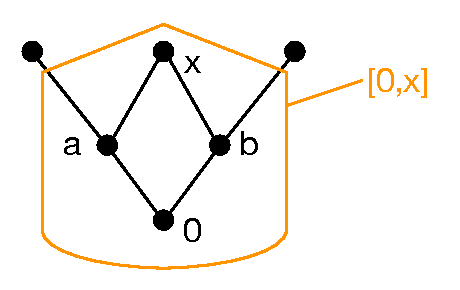
\includegraphics[width=0.4\textwidth]
        {02_higher_combinatorics/pics/LatticeInterval}}}\\
     & $S_f(x) = f(0) + f(a) + f(b) + f(x) $\\
     & $a_n = \sum_{k \leq n} a_k - \sum_{k \leq n-1} a_k =
              S_f(n) - S_f(n-1)$\\
\end{tabular}~\\

\textbf{Problem.}
Given $S_f$, find $f$

\begin{definition}
$(P, \leq)$ is a locally finite poset with a 0-element.
We have a \dt{Möbius function} of $P$ $\mu: P\times P \rightarrow \mathbb{R}$
if
\[
  \forall x,y \in P: \sum_{z\in [x, y]} \mu(z,y) = \delta_{x,y} =
    \begin{cases}
      1 & \text{if } x = y \\
      0 & \text{otherwise}
    \end{cases}
\]
\end{definition}

\Remark.
$\mu$ uniquely determined, $x \not\leq y \implies \mu(x,y) = 0$

\textbf{Example.}
\begin{align*}
  [x,x] & = \{x\}, && \mu(x,x) = 1 \\
  [x,y] &= \{x,y\} && \mu(x,y) + \mu(y,y) = 0 \\
        &          && \mu(y,y) = 1 \implies \mu(x,y) = -1 \\
\end{align*}

\textbf{Example.}
$(\mathbb{N}, \leq)$: $\mu(n,n) = 1,\; \mu(n,n+1) = -1$

$[n,n+2] = \{n,n+1, n+2\}:$

\[
\begin{matrix}
  \mu(n,n+2) & + & \mu(n+1,n+2) & + & \mu(n+2, n+2) & = 0 \\
  0 & -&1 &+&1 & = 0
\end{matrix}
\]
$ m \geq n+2 \implies \mu(n,m) = 0$

\begin{center}
    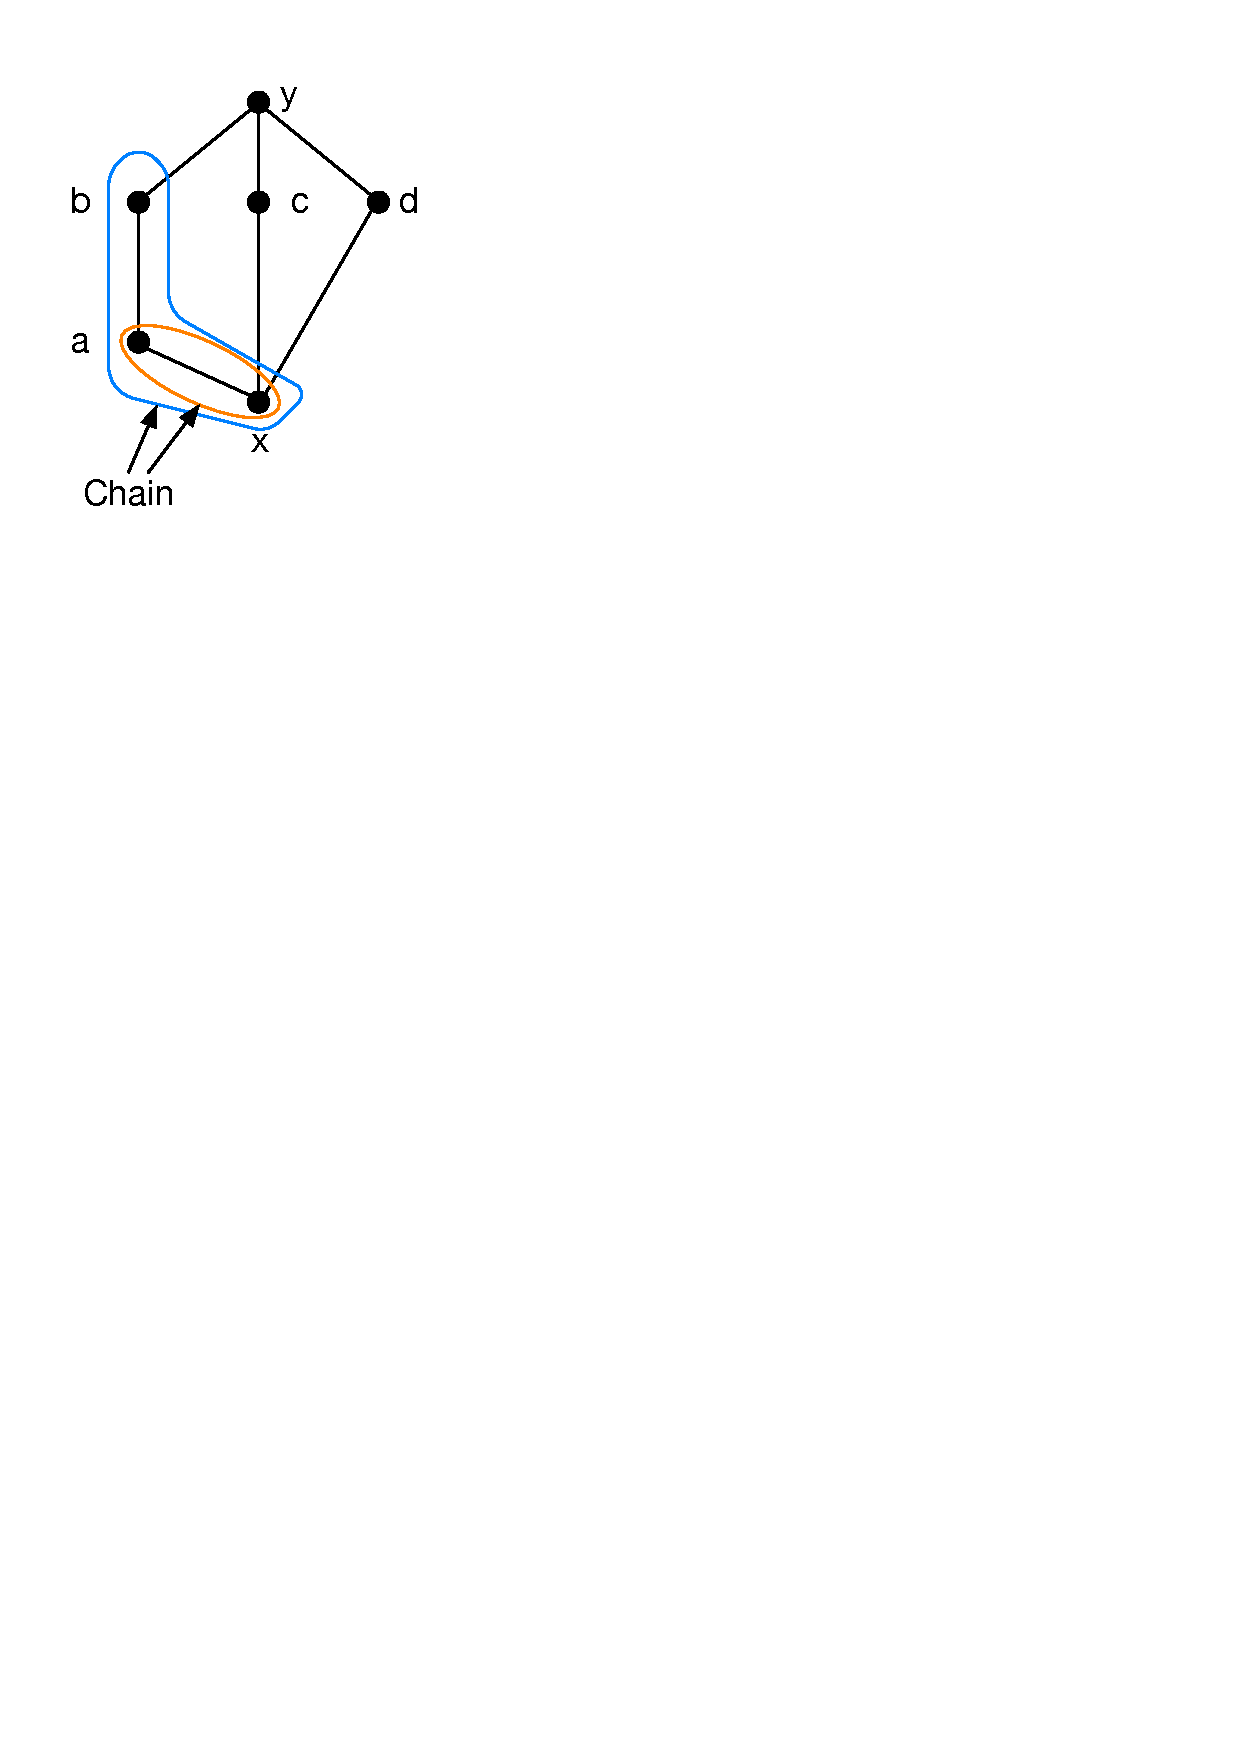
\includegraphics[width=0.3\textwidth]
      {02_higher_combinatorics/pics/LatticeMoebiusFunction}
\end{center}
\begin{align*}
    \mu(x,x) &= \mu(a,a) = \mu(b,b) = \mu(c,c) = \mu(d,d) = \mu(y,y) = 1\\
    \textcolor{orange}{\mu(x,a)} &= \mu(x,c) = \mu(x,d) = \mu(a,b) = \mu(b,y) = \mu(c,y) = \mu(d,y) = -1\\
    \textcolor{aqua}{\mu(x,b)} &= 0, \mu(a,y) = 0\\
    \mu(x,y)&:  \underbrace{\mu(x,y)}_{2}
              + \underbrace{\mu(a,y)}_{0}
              + \underbrace{\mu(b,y)}_{-1}
              + \underbrace{\mu(c,y)}_{-1}
              + \underbrace{\mu(d,y)}_{-1}
              + \underbrace{\mu(y,y)}_{1} = \delta_{x,y} = 0 \\
\end{align*}
\Theorem.
$(P_1, \leq_1), (P_2, \leq_2)$, locally finite poset, with 0-element.
We define $(P, \leq)$ as
\[
  P = P_1 \times P_2, (x_1,x_2) \leq (y_1, y_2) :\implies x_1 \leq_1 y_1 \text{ and } x_2 \leq_2 y_2
\]

$\Rightarrow (P, \leq)$ is locally finite poset with 0-element ($=(0_1, 0_2)$) with a Möbius function $\mu: P\times P \rightarrow \mathbb{R}$
\begin{align*}
  \mu ( (x_1, x_2), (y_1,y_2)) &= \mu_1(x_1,y_1) \cdot \mu_2(x_2,y_2) \\
  (P, \leq) &= (P_1, \leq_1) \cdot (P_2, \leq_2)
\end{align*}

\textbf{Example.}
We have a set $M = \{a_1, \ldots , a_n\}$. We claim that
\[
  (2^M, \subseteq) \cong ( \{0,1\}, \leq)^n
\]

E.g.: $n = 5: A = \{a_2,a_5\}, B= \{a_1, a_2, a_3, a_5\},\; A, B \in 2^M$
\begin{align*}
  A &\hat{=} (0,1,0,0,1) \\
  B &\hat{=} (1,1,1,0,1) \\
  A \subseteq B &\hat{=} (0,1,0,0,1) \subseteq (1,1,1,0,1) \\
\end{align*}
\[
  x \in A \rightarrow e_{x,A} = 1 \Rightarrow  e_{x,B} = 1 \implies x \in B\\
\]

Remark that: $e_{x,A} = 1 \Rightarrow e_{x,B} = 1$ is equal to $e_{x,A} \leq e_{x,B}$

\[
    ( \{0,1\}, \leq): \mu(0,0) = \mu(1,1) = 1, \mu(0,1) = -1, \mu(1,0) = 0
\]
\begin{align*}
    \mu(A,B) &= \mu(01001, 11101) = \mu(0,1) \mu(1,1) \mu(0,1) \mu(0,0) \mu(1,1) \\
    &= -1 +1 -1 +1 +1 \\
    &= 1
\end{align*}

We see that:
$A\not\subseteq B \Rightarrow \mu(A,B) = 0$,
$A\subseteq B \Rightarrow (-1)^{|B| - |A|}$.

\Theorem.
(Möbius inversion)
$(P, \leq)$ is a locally, finite poset with a 0-element.
$\mu: P \times P \rightarrow \mathbb{R}$ is the Möbius function of $(P, \leq)$.

Let the sum function $S_f: P \rightarrow \mathbb{R}$ of $f: P \rightarrow \mathbb{R}$ be given by:
\[
  S_f(x) = \sum_{z \in [0,x]} f(z).
\]
\[
 \Rightarrow f(x) = \sum_{z \in [0,x]} S_f(z) * \mu(z,x)
\]

\textbf{Example.}
$(\mathbb{N}, \leq)$, $f: \mathbb{N} \rightarrow \mathbb{R}$, $S_f(n) = \displaystyle{\sum_{k=0}^{n} f(k)}$

\[
  f(n) = \sum_{k=0}^{n} S_f(k) \mu(k,n) = S_f(n) - S_f(n-1)
\]

\Proof.
\begin{minipage}[t]{0.6\textwidth}
  \begin{align*}
      \sum_{z \in [0,x]} S_f(z) * \mu(z,x)
      &= \sum_{z \in [0,x]} \sum_{u \in [0,x]} f(u) \mu(z,x) \\
      &= \sum_{u \in [0,x]} \sum_{z \in [0,x]} f(u) \mu(z,x) \\
      &= \sum_{u \in [0,x]} f(u) \sum_{z \in [0,x]} \mu(z,x) \\
      &= \sum_{u \in [0,x]} f(u) \delta_{u,x} \\
      &= f(x)
  \end{align*}
\end{minipage}
\begin{minipage}[t]{0.3\textwidth}
  \vspace{1.2cm}
  \begin{center}
    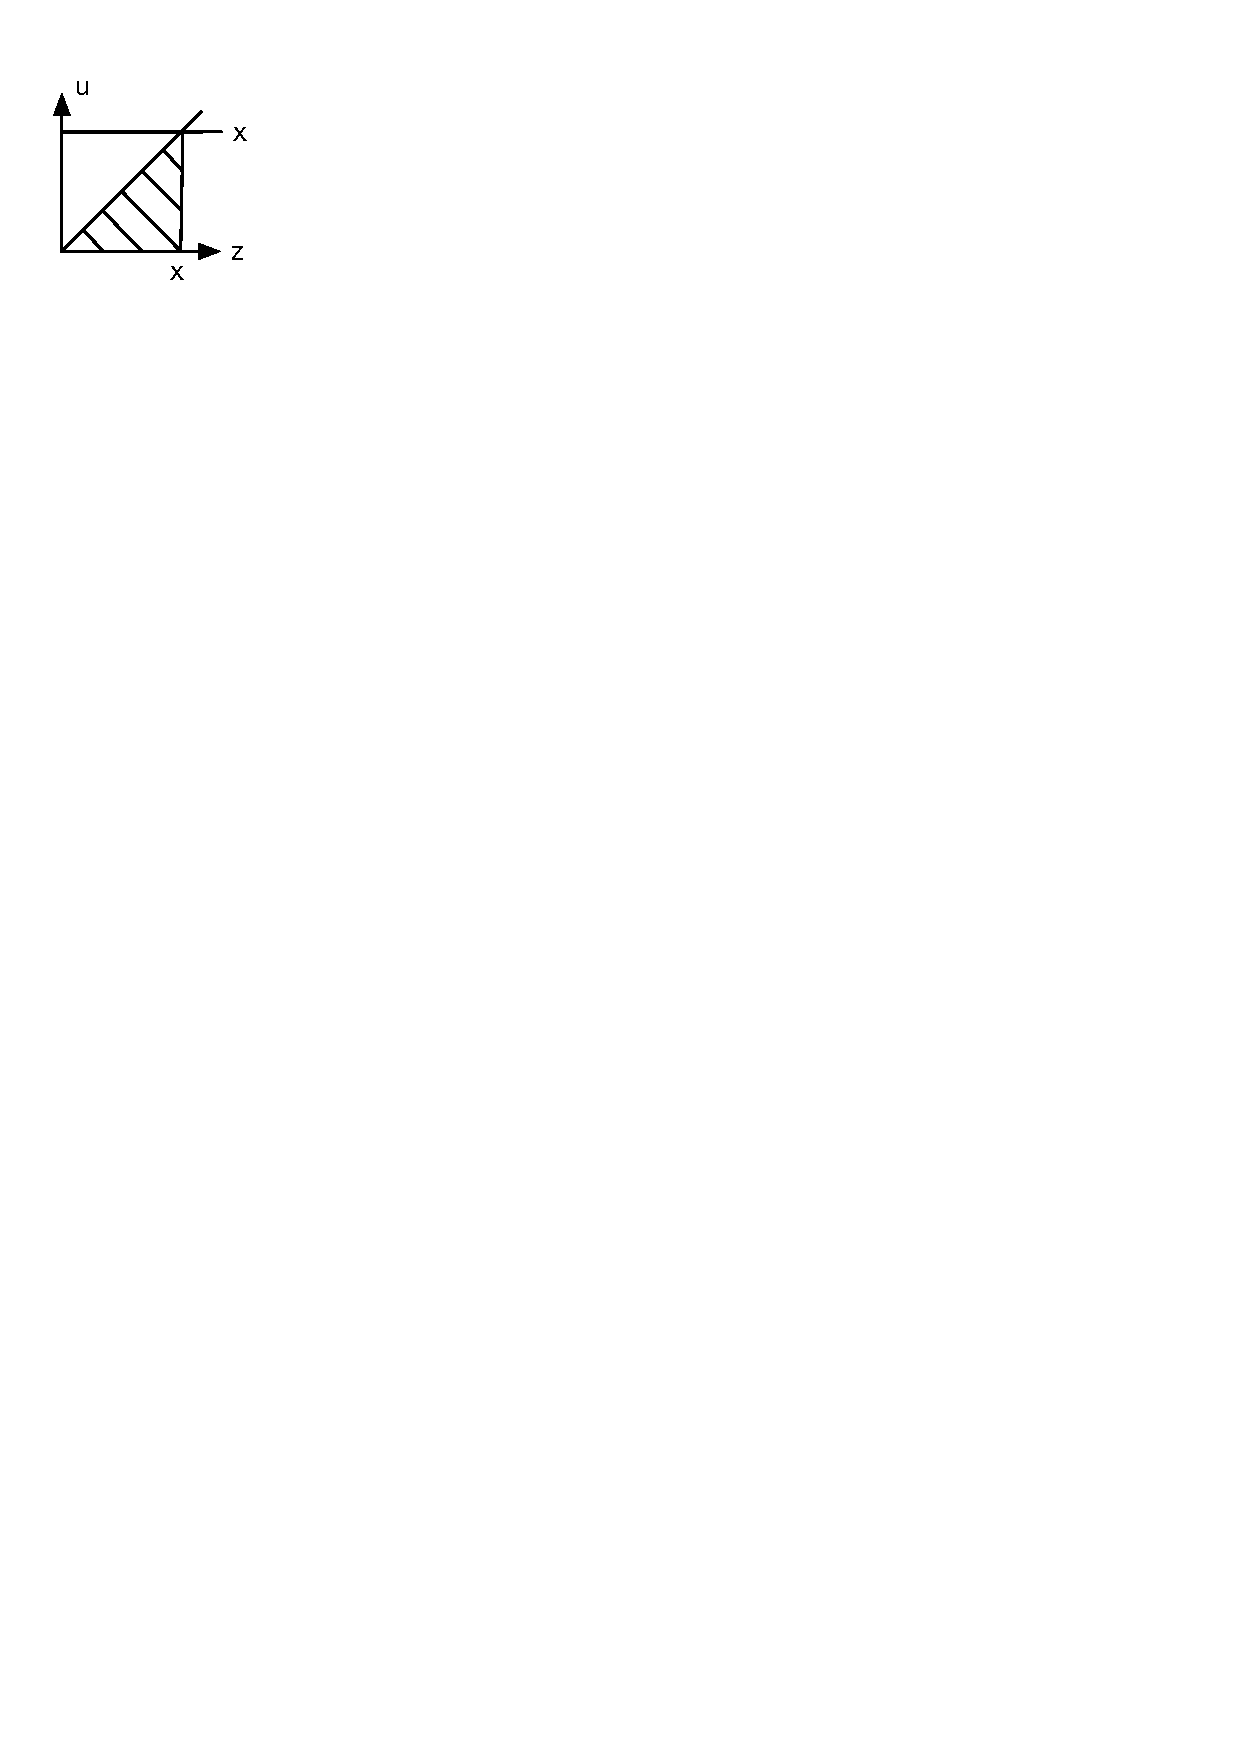
\includegraphics[width=0.8\textwidth]
      {02_higher_combinatorics/pics/MoebiusSum}
  \end{center}
\end{minipage}

\textbf{Example}.
\lecturedate[\baselineskip]{2013-11-29}
Sets $A_1, A_2, \ldots A_m \subseteq M$. We take the powerset of set of indices $(2^{\{1,2, \ldots , m\}}, \supseteq)$. 
Note that the Möbius Function only depends on the structure of the order. 

\[
  \mu (A,B) = \begin{cases} 
    (-1)^{|B| - |A|} &, A\supseteq B\\ 
    0                & \text{, otherwise}
  \end{cases}
\]

\begin{gather*}
  I \subseteq \{ 1,2, \ldots, m\}, \\
  f(I) = \left| \bigcap_{i\in I} A_i \cap 
    \bigcap_{j \in \{1,\ldots ,m\} \backslash I} \bar{A}_j \right| \\
  S_f(I) = \sum_{J \supseteq I} f(J) = \left| \bigcap_{i\in I} A_i  \right| \\
  \left[ S_f(x) = \sum_{z\leq x} f(z) \right]
\end{gather*}

\begin{align*}
  f(I) &= \sum_{J \supseteq I} S_f(I) \mu(J,I) \\
    &= \sum_{J \supseteq I} (-1)^{|J| - |I|} * \left| \bigcap_{i\in I} A_i \right| \\
  f(\varnothing) &= \left| \bigcap_{j \in \{1,\ldots ,m\}} \bar{A}_j \right| \\
    &= \sum_{j \in \{1,\ldots ,m\}} (-1)^{|J|} \left| \bigcap_{j \in J} A_j \right|
\end{align*}

\textbf{Example.}
Poset $(\mathbb{N}^{+}, \mid)$.
We can say if n is a product $n = p_1^{g_1} \ldots p_r^{g_r}$ and $m$ is the product $m = p_1^{f_1} \ldots p_r^{f_r}$. This implies 
\[
  m|n \iff \forall f_i \leq g_i
\]

The number theoretical number order $(\mathbb{N}^{+}, \mid)$ is isomorphic to $(\mathbb{N} \times \mathbb{N} \times \ldots , \leq)$

\begin{align*}
  \mu(n) =& \mu_{|}(1,n) = \mu_{\leq}(0,g_1) \leq \mu_{\leq}(0,g_2) \ldots * \mu_{\leq}(0,g_r) \\
    =& \begin{cases} 
      1 & \text{if } n=1 \\
      (-1)^r & \text{if } n = p_1 p_2 \ldots p_r \text( square-free) \\
       & \text{if } \exists p\in \mathbb{P}: p^2|n
     \end{cases} \\
  m \not| n: &\mu(m,n) = 0 \\
  m \mid n:  &\mu(m,n) = \mu(1, \frac{n}{m}) \\
\end{align*}

\TODO{Hassediagram, [3,18], show when m|n we can divide}

\begin{align*}
  f: &\mathbb{N}^{+} \rightarrow \mathbb{R}, \\
  S_f(n) =& \sum_{d\mid n} f(d) \Rightarrow f(n) = \sum_{d\mid n} S_f(d)\mu\left(\frac{n}{d}\right)
\end{align*}

\subsection{Lattices}
\begin{definition}
Let $(P, \leq)$ be a poset, and $x,a,b \in P: a\leq x \leq b$. Furthermore say $a$ is a lower bound for $x$, and $b$ be an upper bound for $x$.

The smallest common upper bound of $x,y \in P: x \vee y$ ("$x$ join $y$").

The greatest common lower bound of $x,y \in P: x \wedge y$ ("$x$ meet $y$").

\begin{align*}
    X \subseteq P: &\bigvee_{x \in X} x \text{ join of } X, 
        & \bigwedge_{x \in X} x \text{ meet of } X 
\end{align*}
\end{definition}

\begin{definition}
A poset $(L, \leq)$ is a \dt{lattice} if $\forall x,y \in L \; \exists x \wedge y, x \vee y$.

If only $x \wedge y$ exists: meet-semilattice. 

If only $x \vee y$ exists: join-semilattice. 

\TODO{diagramm of lattice}

If $\forall X \subseteq L : \bigwedge_{x \in X} x, \bigvee_{x \in X} x$ exist, $\rightarrow$ complete lattice
\end{definition}

\textbf{Example.}
\begin{align*}
  (2^M, \subseteq) \\
  A\vee B = A \cap B, \\
  A\wedge B = A \cup B
\end{align*}

\begin{align*}
  (\mathbb{N}, \mid) \\
  x \vee y = gcd(x,y), \\
  x \vee y = lcm(x,y)
\end{align*}

\textbf{Remember.}
$(L, \vee, \wedge): \vee, \wedge$ are both associative, commutative, idempotent ($a\wedge a = a$, $a\vee a = a$). 

absorbtion laws: $a \wedge(a \vee b) = a = a \vee ( a \wedge b)$, $0 \vee a = a$, $1 \wedge a = a$. 

Furthermore we have semigroups $(L, \wedge)$ and $(L, \vee)$.

\Lemma.
If $L$ is a lattice, and $x,y,s,t \in L$. And $s$ is a common upper bound $x \leq s, y \leq s \Rightarrow x \vee y \leq s$. 
And $x \geq t, y \geq t \Rightarrow x \wedge y \geq t$. 

\Remark.
\[
  a \leq b \Leftrightarrow a \vee b = b \Leftrightarrow a \wedge b = a
\]

\Lemma.
$L$ finite meet-semilattice with 1-element. Then $L$ is a lattice.

\Proof.
Assume $x,y \in L$, Set $B = \{u \in L \mid x \leq u \wedge y \leq u\}$. 

\begin{align*}
  x \leq 1, y \leq 1
    \Rightarrow 1 \in B \Rightarrow B \neq \varnothing, |B| < \infty \\
  \Rightarrow B= \{u_1, u_2 \ldots , u_m\}: 
    u:= u_1 \wedge u_2 \wedge \ldots \wedge u_m \\
  \Rightarrow u \in B \\
  u_i \geq x, u_i \geq y \Rightarrow u_i \geq x \wedge y
\end{align*}


\Lemma.
\begin{align*}
  &x \leq s, y \leq s \\
  &x \leq t, y \leq t \\
  &\Rightarrow x \leq s \wedge t, y \leq s \wedge t
\end{align*}

\Proof.
$s \wedge t$ greatest common lower bound of $s,t$. 
$x,y$ are lower bounds of $s,t$ $\Rightarrow$ $x \leq s \wedge t, y \leq s \wedge t$. 

\textbf{Example.}
$\Pi_n$ is the set of partitions of $\{1,2,..., n\}$. 
\[
    (\Pi_n, \leq): A \leq B: \iff \text{$A$ is refinement of $B$}
\]
\TODO{Table of refinement of B with fancy coloring}

We claim $(\Pi_n, \leq)$ is a lattice. 
It is easy to show that $(\Pi_n, \leq)$ is a poset. 

\begin{align*}
  \text{1-el}: & \text{ 1-block partition} \\
  \text{0-el}: & \text{ each block of size 1} \\
  \alpha, \beta \in \Pi_n: & \;\alpha \wedge \beta: i,j \in \{1,2,\ldots,n\} 
    \text{ in the same block } \\
    & \implies \text{ they are in the same block of both $\alpha$ and $\beta$} \\
  &\Rightarrow \Pi_n \text{ is a lattice}
\end{align*}

\Theorem.
$L$ is a lattice with 0-element and 1 element, $b \in L\backslash \{1\}$
\begin{align*}
    \Rightarrow \mu(0,1) = -\sum_{x: x\wedge b = 0, x \neq 0} \mu(x,1) (*)
\end{align*}

\Proof.
$(*) \Leftrightarrow \sum_{x: x\wedge b = 0} \mu(x,1) = 0$
, since $0 \wedge b = 0$

Let $y \leq b$, and we set $N(y) = \sum_{x: x\wedge b=y} \mu(x,1)$.

\begin{align*}
  S(b) &:= \sum_{y: y \leq b} N(y) \\
    & = \sum_{y: y \leq b} \sum_{x: x\wedge b=y} \mu(x,1) \\
    & = \sum_{x,y: x \wedge b = y} \mu(x,1)
\end{align*}

\textbf{Note.}
\begin{align*}
  &\forall x \in L \; \exists!\, y \in L : x \wedge b = y \\
  &\Rightarrow \forall x \in L: \mu(x,1) \text{ occurs exactly once in $S(b)$} \\
  &\Rightarrow S(b) = \sum_{x \in L} \mu(x,1) = \sum_{x \in [0,1]} \mu(x,1) = \delta_{0,1} = 0 \\
  &\Rightarrow \sum_{y \in [0,b]} N(y) = 0 \\
  &\stackrel{\text{MIF}}{\Rightarrow} N(b) = \sum_{y \leq b} S(y) \mu(y,b) = 0\\
  &N(0) = 0, \text{ but } N(0) = \sum_{x:x \wedge b = 0} \mu(x,1) = 0 \\
\end{align*}

With the Note in mind, we can now compute for the previous example
\[
    \mu( 0_{\Pi_n}, 1_{\Pi_n}) = (-1)^{n-1} (n-1)!
\]






